\begin{center}
	{\fboxrule=4pt \fbox{\fboxrule=1pt
		\fbox{\LARGE{\bfseries Virtualización con VirtualBox y Vagrant}}}} \\
	\addcontentsline{toc}{section}{Virtualización con VirtualBox y Vagrant}
	\setcounter{section}{1}
	\setcounter{subsection}{0}
	\rule{15cm}{0pt} \\
\end{center}

\subsection{Enunciado VirtualBox}

\begin{ejer}
    \par El objetivo de esta práctica es gestionar máquinas virtuales con el shells de VirtualBox. 
	Para ello se deberán realizar las siguientes tareas:
	\begin{itemize}
		\item Crear una VM mediante el Shell de VirtualBox, Vboxmanage: 
		\begin{itemize}
			\item 1GB de ram, 2 cpus, 8 GB de disco duro SATA.
		\end{itemize}
		\item Instalar ubuntu-server en la máquina. Instalarle el servicio nginx a la máquina. 
		\item Instalar ubuntu-desktop en otra máquina. Instalar un navegador web. 
		\item Comprobar que podemos acceder al servidor web desde un navegador en el host.
		\item Comprobar que podemos acceder al servidor web desde un navegador en la máquina guest desktop.
		\item Transformar el disco de la máquina de formato .vdi a formato qcow2. 
		\item Redimensionar la maquina original servidor de VirtualBox con la utilidad \textbf{Vboxmanage:} 2GB de RAM y 10GB disco duro. 
		\item Destruir las máquinas virtuales (utilizando comandos).
	\end{itemize}
\end{ejer}


\subsection{Pasos VirtualBox}

%%%%%%%%%%%%%%%%%%%%%%%%%%%%%%%%%%%%%%%%%%%%%%%%%%%%%%%%%%%%%%%%%%%%%%%%%%%%%%%%%%%%%%%%%%%%%%%%%%%%%%%%%%%%%%%%%%%%%%%%%%%%%%%%%%%%%%%%%%%%%%
\subsubsection{Crear una VM mediante el Shell de VirtualBox, Vboxmanage: 1GB de ram, 2 cpus, 8 GB de disco duro SATA.}

\par \textbf{El primer paso} para crear una máquina virtual es usar el comando \texttt{createvm},
que su única función es construir un archivo \texttt{XML} que define la nueva maquina virtual.
La opción \texttt{--register} sirve para importar la definición de la maquina virtual
dentro de Oracle VM VirtualBox, aunque también se puede realizar con el comando 
\texttt{registervm}. El uso del parámetro \texttt{--name} es obligatorio y en este caso 
nombraré mi primera VM como \textit{teii-server}, adicionalmente incluyo el tipo de 
sistema operativo que tengo intención de instalar en esta máquina, como se muestra en 
la Figura \ref{fig:vboxmanage-createvm}.
%%% IMAGEN VBOXMANAGE CREATEVM %%%
\begin{figure}[H]
    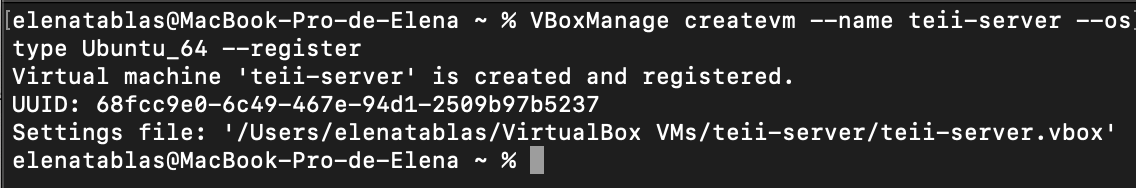
\includegraphics[width=\textwidth]{vboxmanage-createvm}
    \centering
    \caption{Definición e importación de la VM \textit{teii-server} dentro de \texttt{VirtualBox}.}
    \label{fig:vboxmanage-createvm}
 \end{figure}
\par Esta máquina virtual está vacía, en los siguientes pasos tengo que 
configurar la CPU, RAM, red y el disco duro. Además, en la siguiente sección 
instalo el sistema operativo. 
%%% IMAGEN VBOXMANAGE SHOWVMINFO INICIAL%%%
\begin{figure}[H]
    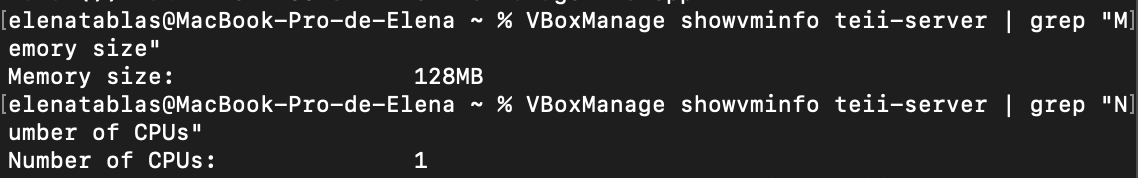
\includegraphics[width=\textwidth]{vboxmanage-showvminfo-inicial}
    \centering
    \caption{Información inicial de la \texttt{VM} \textit{teii-server}.}
    \label{fig:vboxmanage-showvminfo-inicial}
 \end{figure}
\par El comando \texttt{showvminfo} muestra la 
información de la VM, en este caso es la configuración inicial por defecto y 
se puede comprobar en la Figura \ref{fig:vboxmanage-showvminfo-inicial} como la configuración impuesta no es la que quiero.
Por tanto, en \textbf{el segundo paso} modifico el número de CPUs y el tamaño de la RAM con el comando 
\texttt{modifyvm} y compruebo que la información se ha configurado correctamente en la Figura \ref{fig:vboxmanage-showvminfo-segundo-paso}.
\begin{listing}[style=consola]
    $ VBoxManage modifyvm teii-server --cpus 2 --memory 1024
\end{listing}
%%% IMAGEN VBOXMANAGE SHOWVMINFO SEGUNDO PASO %%%
\begin{figure}[H]
    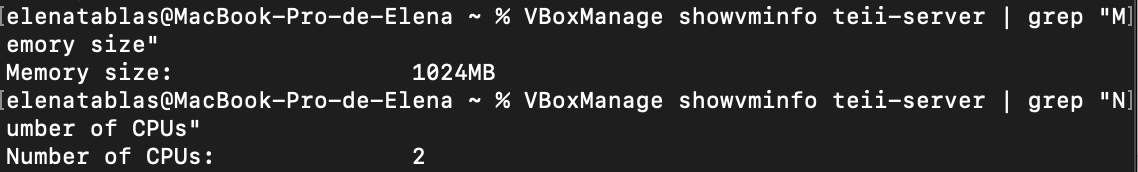
\includegraphics[width=\textwidth]{vboxmanage-showvminfo-segundo-paso}
    \centering
    \caption{Información modificada de la VM \textit{teii-server}.}
    \label{fig:vboxmanage-showvminfo-segundo-paso}
 \end{figure}
\par Además, configuro el adaptador de red con el mismo comando que antes para que 
la máquina virtual pueda interactuar con el host y otras máquinas virtuales conectadas
a la misma red. Este paso es útil para que otras máquinas puedan acceder a este servidor web con servicio \texttt{nginx}.
\begin{listing}[style=consola]
    $ VBoxManage modifyvm teii-server --nic1 hostonly --hostonlyadapter1 vboxnet2
\end{listing}

\par \textbf{El tercer paso} es la creación de un disco duro virtual. Como en un 
ordenador real, la VM necesita uno para poder bootear y almacenar información del sistema y del usuario. 
Para ello debo utilizar tres comandos.
\begin{itemize}
    \item Comando \texttt{createhd}: crea una imagen de disco en formato \texttt{VDI}.
    Si el directorio que se le pasa como parámetro no existe, \texttt{VirtualBox} lo crea.
    %%% IMAGEN VBOXMANAGE CREATEHD %%%
    \begin{figure}[H]
        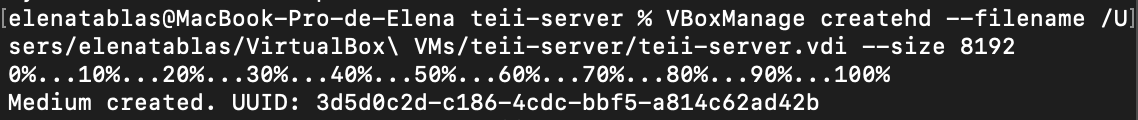
\includegraphics[width=\textwidth]{vboxmanage-createhd}
        \centering
        \caption{Creación de una imagen de disco de 8GB.}
        \label{fig:vboxmanage-createhd}
    \end{figure}
    \item Comando \texttt{storagectl}: añade un controladore de alamacenamiento, en este caso elijo \texttt{Serial ATA (SATA)}.
\begin{listing}[style=consola]
    $ VBoxManage storagectl teii-server  --name "SATA Controller" --add sata --bootable on
\end{listing}
    \item Comando \texttt{storageattach}: asocia el nuevo disco duro virtual con el controlador.
\begin{listing}[style=consola]
    $ VBoxManage storageattach teii-server --storagectl "SATA Controller" --port 0 --device 0 --type hdd --medium /Users/elenatablas/VirtualBox\ VMs/teii-server/teii-server.vdi
\end{listing}
\end{itemize}
\par Compruebo que la información del nuevo disco duro virtual es correcta como indica la Figura \ref{fig:vboxmanage-showmediuminfo-inicial}.
%%% IMAGEN VBOXMANAGE SHOWMEDIUMINFO INICIAL %%%
\begin{figure}[H]
    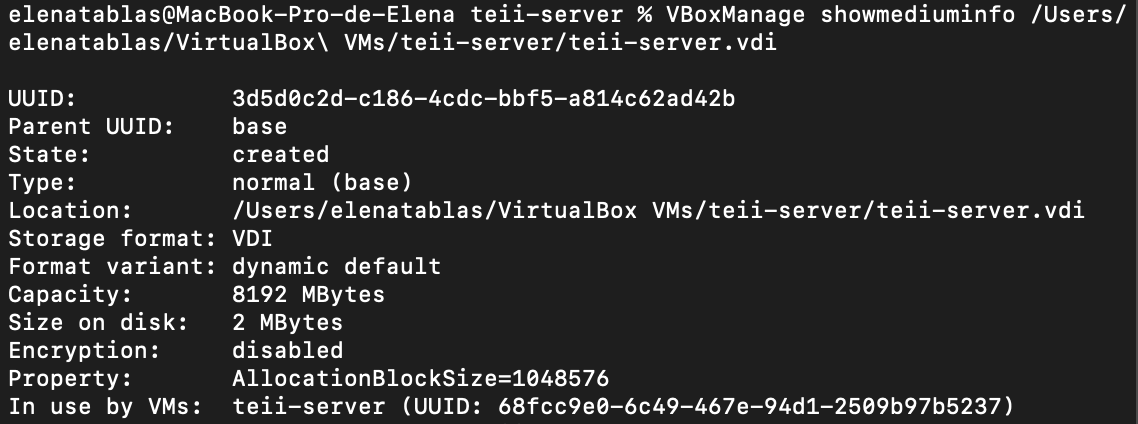
\includegraphics[width=\textwidth]{vboxmanage-showmediuminfo-inicial}
    \centering
    \caption{Información del nuevo disco duro virtual usado en la VM \textit{teii-server}.}
    \label{fig:vboxmanage-showmediuminfo-inicial}
 \end{figure}

%%%%%%%%%%%%%%%%%%%%%%%%%%%%%%%%%%%%%%%%%%%%%%%%%%%%%%%%%%%%%%%%%%%%%%%%%%%%%%%%%%%%%%%%%%%%%%%%%%%%%%%%%%%%%%%%%%%%%%%%%%%%%%%%%%%%%%%%%%%%%%
\subsubsection{Instalar ubuntu-server en la máquina. Instalarle el servicio nginx a la máquina.}
\par \textbf{El primer paso} es descargar la imagen iso en el ordenador, en este caso he descargado
la versión \texttt{ubuntu-16.04.7-server-amd64}.
\par \textbf{El siguiente paso} es configurar el arranque de la maquina virtual para que 
la instalación empiece cuando la VM arranque por primera vez. 
\par \textbf{El tercer paso} es crear un dispositivo CD/DVD virtual y conectarlo. Además, 
necesita un controlador. Utilizaré los mismos comandos descritos cuando la creación del disco duro virtual.

\begin{listing}[style=consola]
    $ VBoxManage storagectl teii-server --name "IDE Controller" --add ide
    $ VBoxManage storageattach teii-server --storagectl "IDE Controller" --port 0  --device 0 --type dvddrive --medium /Users/elenatablas/Downloads/ubuntu-16.04.7-server-amd64.iso
\end{listing}
\par Compruebo que la información del controlador IDE como indica la Figura \ref{fig:vboxmanage-showvminfo-controller}.
%%% IMAGEN VBOXMANAGE SHOWVMINFO IDE CONTROLLER %%%
\begin{figure}[H]
    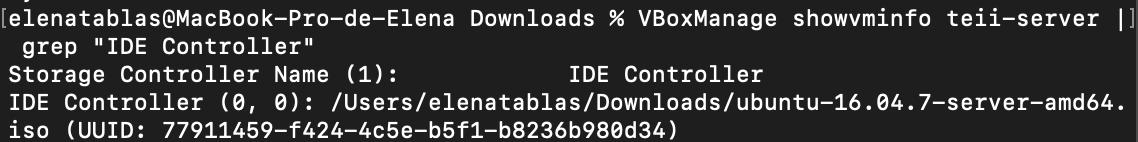
\includegraphics[width=\textwidth]{vboxmanage-showvminfo-controller}
    \centering
    \caption{Información del controlador \texttt{IDE} usado en la VM \textit{teii-server}.}
    \label{fig:vboxmanage-showvminfo-controller}
 \end{figure}
 \par \textbf{El cuarto paso} es arrancar la maquina virtual usando el comando \texttt{startvm}, Figura \ref{fig:vboxmanage-startvm} 
 y configurar los pasos iniciales.
 %%% IMAGEN VBOXMANAGE STARTVM %%%
\begin{figure}[H]
    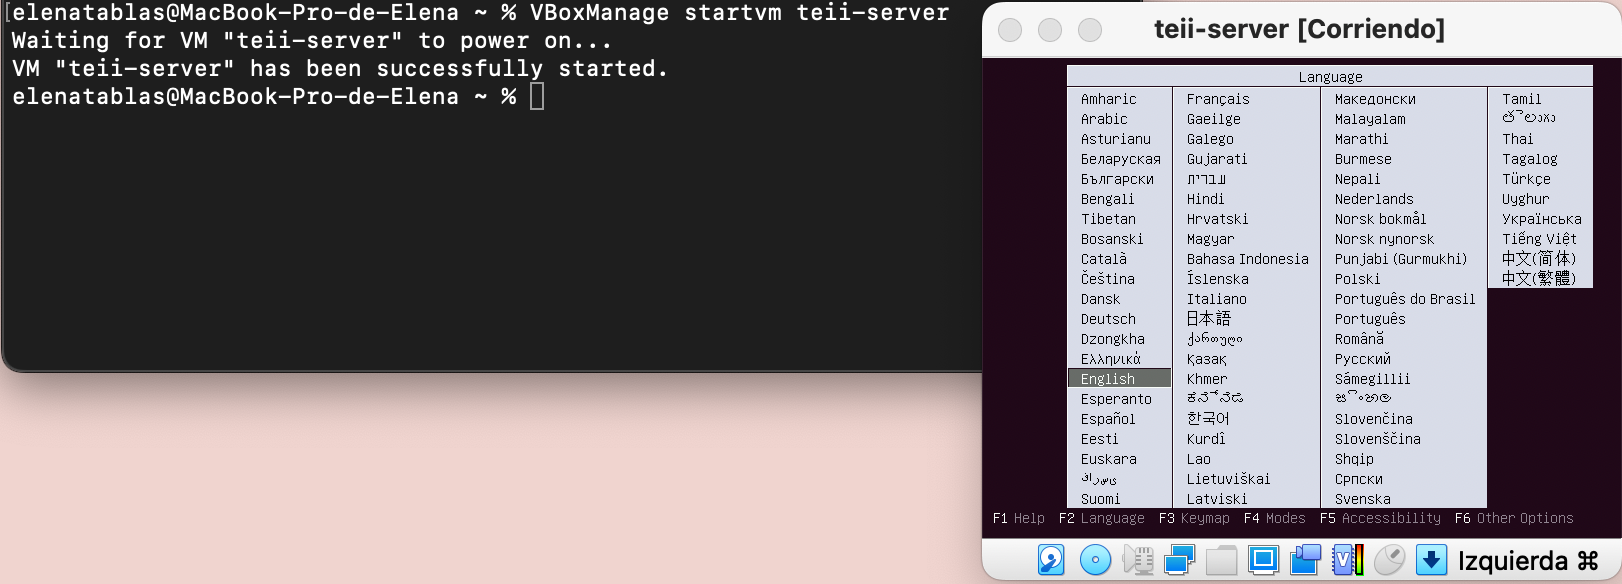
\includegraphics[width=\textwidth]{vboxmanage-startvm}
    \centering
    \caption{Arrancar por primera vez la VM \textit{teii-server}.}
    \label{fig:vboxmanage-startvm}
\end{figure}
\par \textbf{El quinto paso} es apagar la maquina virtual con cualquier comando de estos dos:
\begin{listing}[style=consola]
    $ VBoxManage controlvm teii-server acpipowerbutton
    $ VBoxManage controlvm teii-server poweroff
\end{listing}
\par \textbf{El sexto paso} es eliminar el DVD de la configuración de la VM porque el sistema operativo ya está instalado.
\begin{listing}[style=consola]
    $ VBoxManage storageattach teii-server --storagectl "IDE Controller" --port 0 --device 0 --type dvddrive --medium none
\end{listing}
 %%% IMAGEN VBOXMANAGE STARTVM %%%
 \begin{figure}[H]
    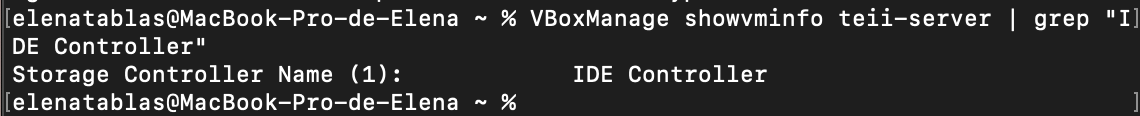
\includegraphics[width=\textwidth]{vboxmanage-eliminar-dvd}
    \centering
    \caption{Eliminación del DVD de la configuración de la VM \textit{teii-server}.}
    \label{fig:vboxmanage-eliminar-dvd}
\end{figure}
\par \textbf{Por último}, arranco la máquina virtual para ver que funciona correctamente e instalo el servicio nginx.
 %%% IMAGEN INSTALACIÓN NGINX %%%
 \begin{figure}[H]
    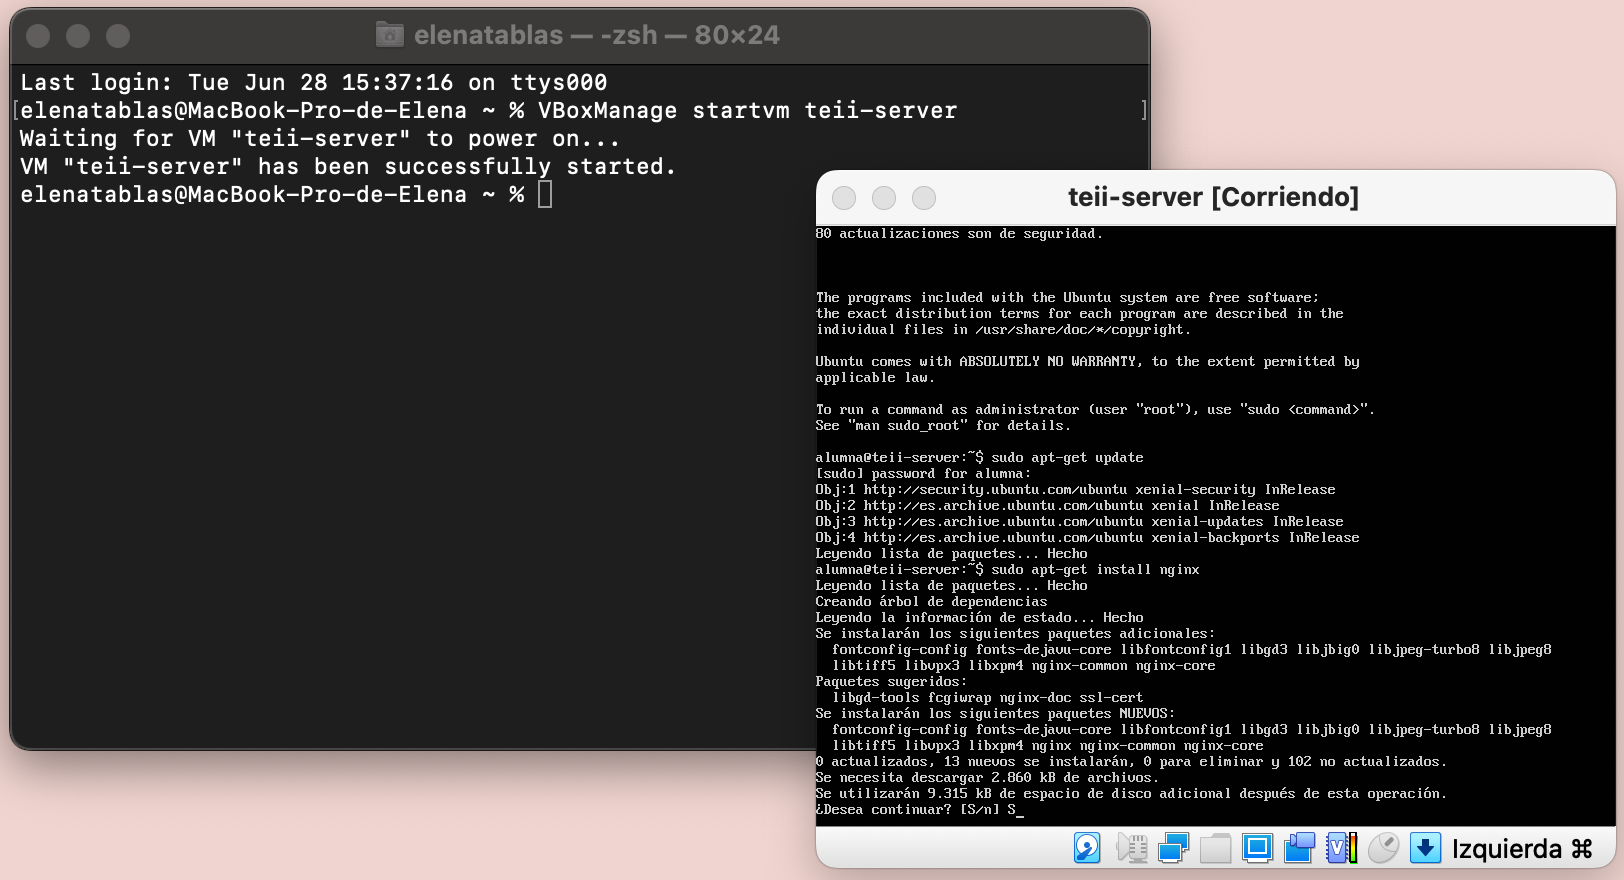
\includegraphics[width=\textwidth]{instalar-nginx}
    \centering
    \caption{Instalación del servicio \texttt{nginx} en la VM \textit{teii-server}.}
    \label{fig:instalar-nginx}
\end{figure}
 
%%%%%%%%%%%%%%%%%%%%%%%%%%%%%%%%%%%%%%%%%%%%%%%%%%%%%%%%%%%%%%%%%%%%%%%%%%%%%%%%%%%%%%%%%%%%%%%%%%%%%%%%%%%%%%%%%%%%%%%%%%%%%%%%%%%%%%%%%%%%%%
\subsubsection{Instalar ubuntu-desktop en otra máquina. Instalar un navegador web.}
\par Los comandos de esta sección son los mismos mencionados en el proceso de creación e instalación de la 
máquina virtual teii-server. Por tanto, las explicaciones se dan por dadas y en está sección 
muestro todos los comandos necesarios y la instalación de un navegador web.
\begin{listing}[style=consola]
    $ VBoxManage createvm --name teii-desktop --ostype Ubuntu_64 --register
    Virtual machine 'teii-desktop' is created and registered.
    UUID: fee2325d-6f39-4053-ac37-d208dbd04e04
    Settings file: '/Users/elenatablas/VirtualBox VMs/teii-desktop/teii-desktop.vbox'
    $ VBoxManage modifyvm teii-desktop --cpus 2 --memory 1024
    $ VBoxManage showvminfo teii-desktop | grep "Memory size"
    Memory size:                 1024MB
    $ VBoxManage showvminfo teii-desktop | grep "Number of CPUs"
    Number of CPUs:              2
    $ VBoxManage modifyvm teii-desktop --nic1 hostonly --hostonlyadapter1 vboxnet2
    $ VBoxManage createhd --filename /Users/elenatablas/VirtualBox\ VMs/teii-desktop/teii-desktop.vdi --size 9216
    0%...10%...20%...30%...40%...50%...60%...70%...80%...90%...100%
    Medium created. UUID: e57978cf-b59a-4373-a1fd-635c176ce949
    $ VBoxManage storagectl teii-desktop --name "SATA Controller" --add sata --bootable on
    $ VBoxManage storageattach teii-desktop --storagectl "SATA Controller" --port 0 --device 0 --type hdd --medium /Users/elenatablas/VirtualBox\ VMs/teii-desktop/teii-desktop.vdi
    $ VBoxManage showmediuminfo /Users/elenatablas/VirtualBox\ VMs/teii-desktop/teii-desktop.vdi
    UUID:           e57978cf-b59a-4373-a1fd-635c176ce949
    Parent UUID:    base
    State:          created
    Type:           normal (base)
    Location:       /Users/elenatablas/VirtualBox VMs/teii-desktop/teii-desktop.vdi
    Storage format: VDI
    Format variant: dynamic default
    Capacity:       9216 MBytes
    Size on disk:   2 MBytes
    Encryption:     disabled
    Property:       AllocationBlockSize=1048576
    In use by VMs:  teii-desktop (UUID: fee2325d-6f39-4053-ac37-d208dbd04e04)
    $ VBoxManage storagectl teii-desktop --name "IDE Controller" --add ide
    $ VBoxManage storageattach teii-desktop --storagectl "IDE Controller" --port 0  --device 0 --type dvddrive --medium /Users/elenatablas/Downloads/ubuntu-16.04.7-desktop-amd64.iso
    $ VBoxManage showvminfo teii-desktop | grep "IDE Controller"
    Storage Controller Name (1):            IDE Controller
    IDE Controller (0, 0): /Users/elenatablas/Downloads/ubuntu-16.04.7-desktop-amd64.iso (UUID: 7f11046c-c18b-4332-8ff6-ddd5d6b63e6e)
    $ VBoxManage startvm teii-desktop
    Waiting for VM "teii-desktop" to power on...
    VM "teii-desktop" has been successfully started.
    $ VBoxManage controlvm teii-desktop poweroff
    $ VBoxManage storageattach teii-desktop --storagectl "IDE Controller" --port 0 --device 0 --type dvddrive --medium none 
    $ VBoxManage startvm teii-desktop
\end{listing}
\par \textbf{Por último}, arranco la máquina virtual para ver que funciona correctamente y veo que viene firefox por defecto.
 %%% IMAGEN INSTALACIÓN FIREFOX %%%
 \begin{figure}[H]
    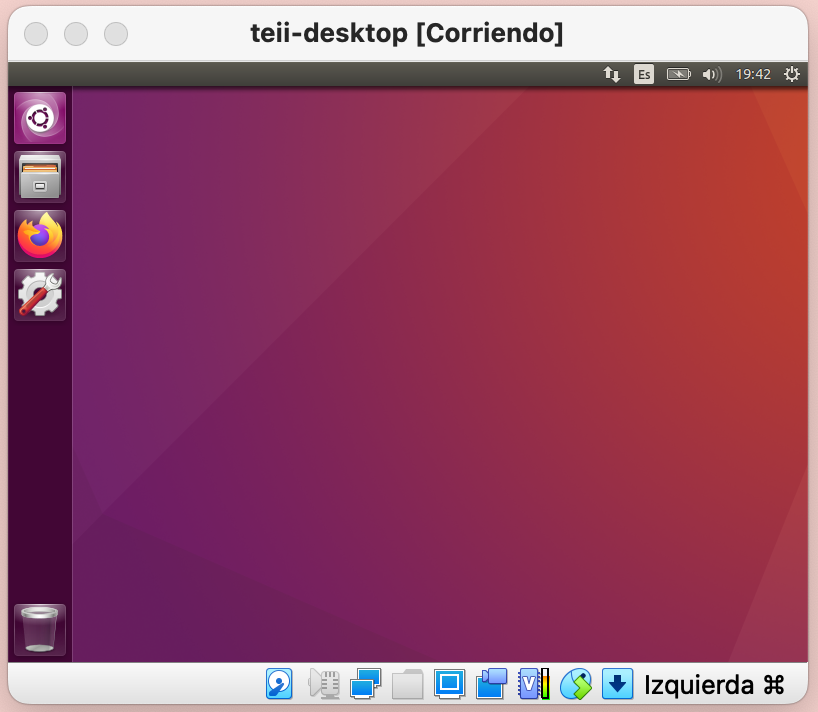
\includegraphics[scale=0.6]{instalar-firefox}
    \centering
    \caption{Instalación del navegador web firefox en la VM \textit{teii-desktop}.}
    \label{fig:instalar-firefox}
\end{figure}

%%%%%%%%%%%%%%%%%%%%%%%%%%%%%%%%%%%%%%%%%%%%%%%%%%%%%%%%%%%%%%%%%%%%%%%%%%%%%%%%%%%%%%%%%%%%%%%%%%%%%%%%%%%%%%%%%%%%%%%%%%%%%%%%%%%%%%%%%%%%%%
\subsubsection{Comprobar que podemos acceder al servidor web desde un navegador en el host.}
\par En la Figura \ref{fig:comprobacion-host}, a la izquierda se puede ver la máquina virtual 
corriendo con el servicio \texttt{nginx} activado y que su dirección IP es la \texttt{192.168.58.3}.
Para acceder al servidor web desde mi host (macOS), abro el navegador web Opera y escribo la url \url{http://192.168.58.3}
como se aprecia en el lado derecho de la Figura \ref{fig:comprobacion-host}.

%%% IMAGEN COMPROBACIÓN HOST %%%
 \begin{figure}[H]
    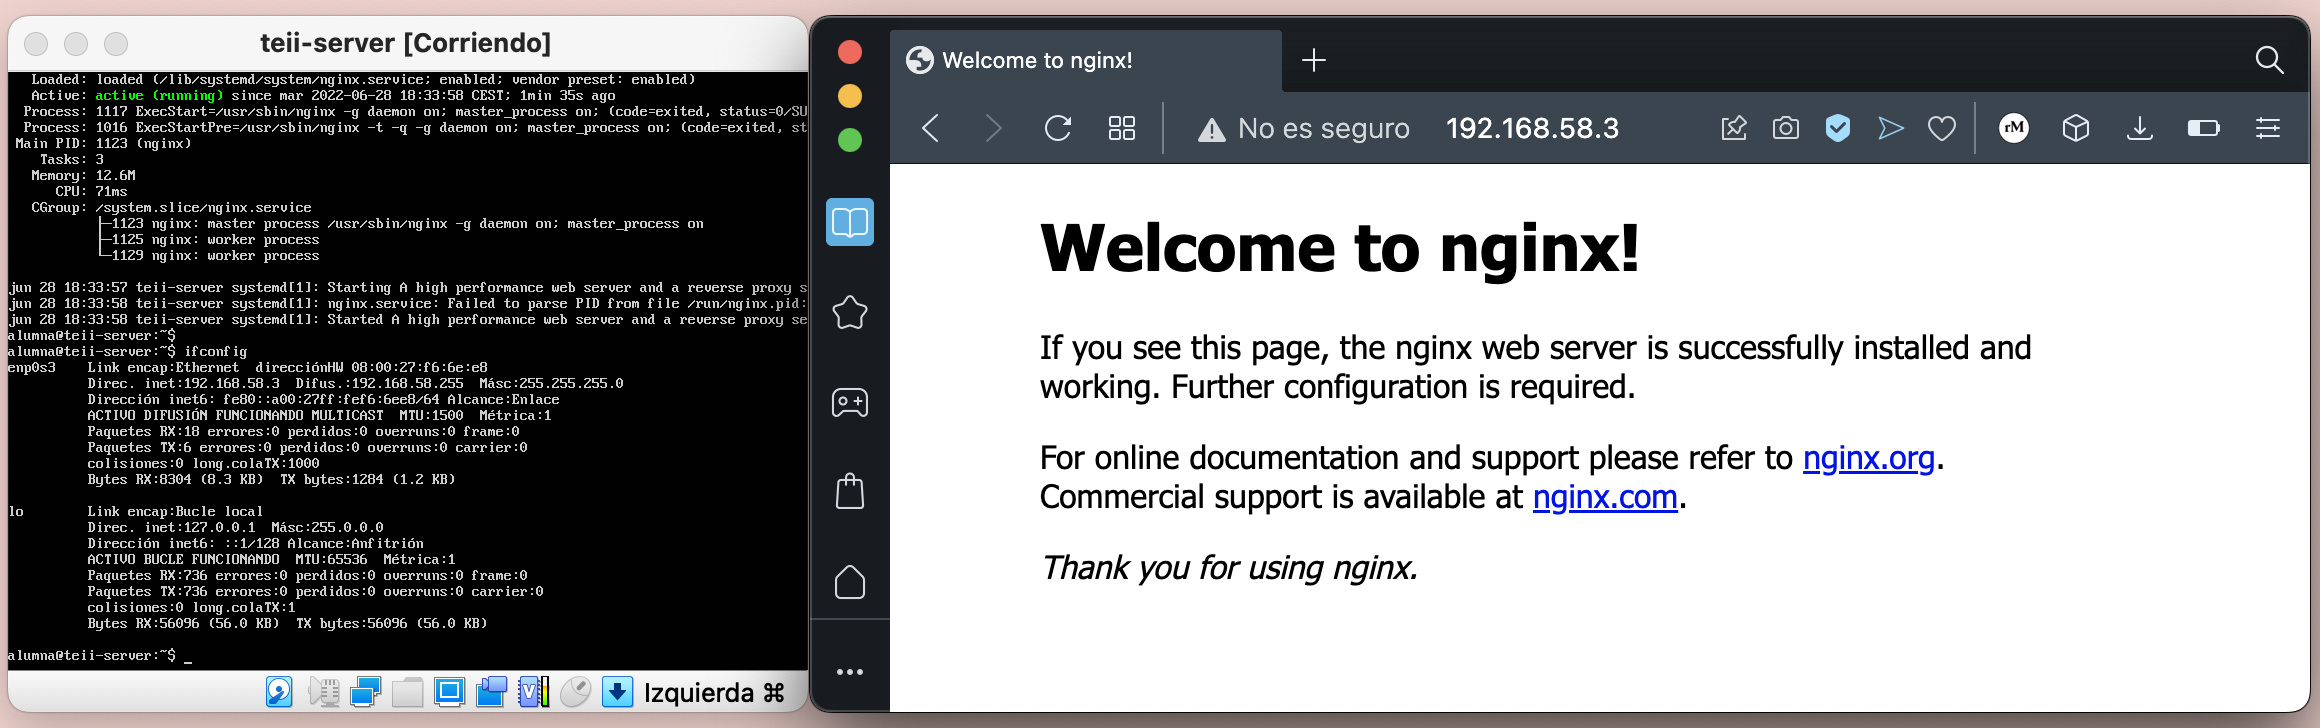
\includegraphics[width=\textwidth]{comprobacion-host}
    \centering
    \caption{Comprobación acceso al servidor web \textit{teii-server} desde el host \texttt{macOS}.}
    \label{fig:comprobacion-host}
\end{figure}


%%%%%%%%%%%%%%%%%%%%%%%%%%%%%%%%%%%%%%%%%%%%%%%%%%%%%%%%%%%%%%%%%%%%%%%%%%%%%%%%%%%%%%%%%%%%%%%%%%%%%%%%%%%%%%%%%%%%%%%%%%%%%%%%%%%%%%%%%%%%%%
\subsubsection{Comprobar que podemos acceder al servidor web desde un navegador en la máquina guest desktop.}

\par En la Figura \ref{fig:comprobacion-desktop}, a la izquierda se puede ver la máquina virtual 
corriendo con el servicio \texttt{nginx} activado y que su dirección IP es la \texttt{192.168.58.3}.
Para acceder al servidor web desde la VM \textit{teii-desktop}, abro el navegador web Firefox y escribo la url \url{http://192.168.58.3}
como se aprecia en el lado derecho de la Figura \ref{fig:comprobacion-desktop}.

%%% IMAGEN COMPROBACIÓN TEII-DESKTOP %%%
 \begin{figure}[H]
    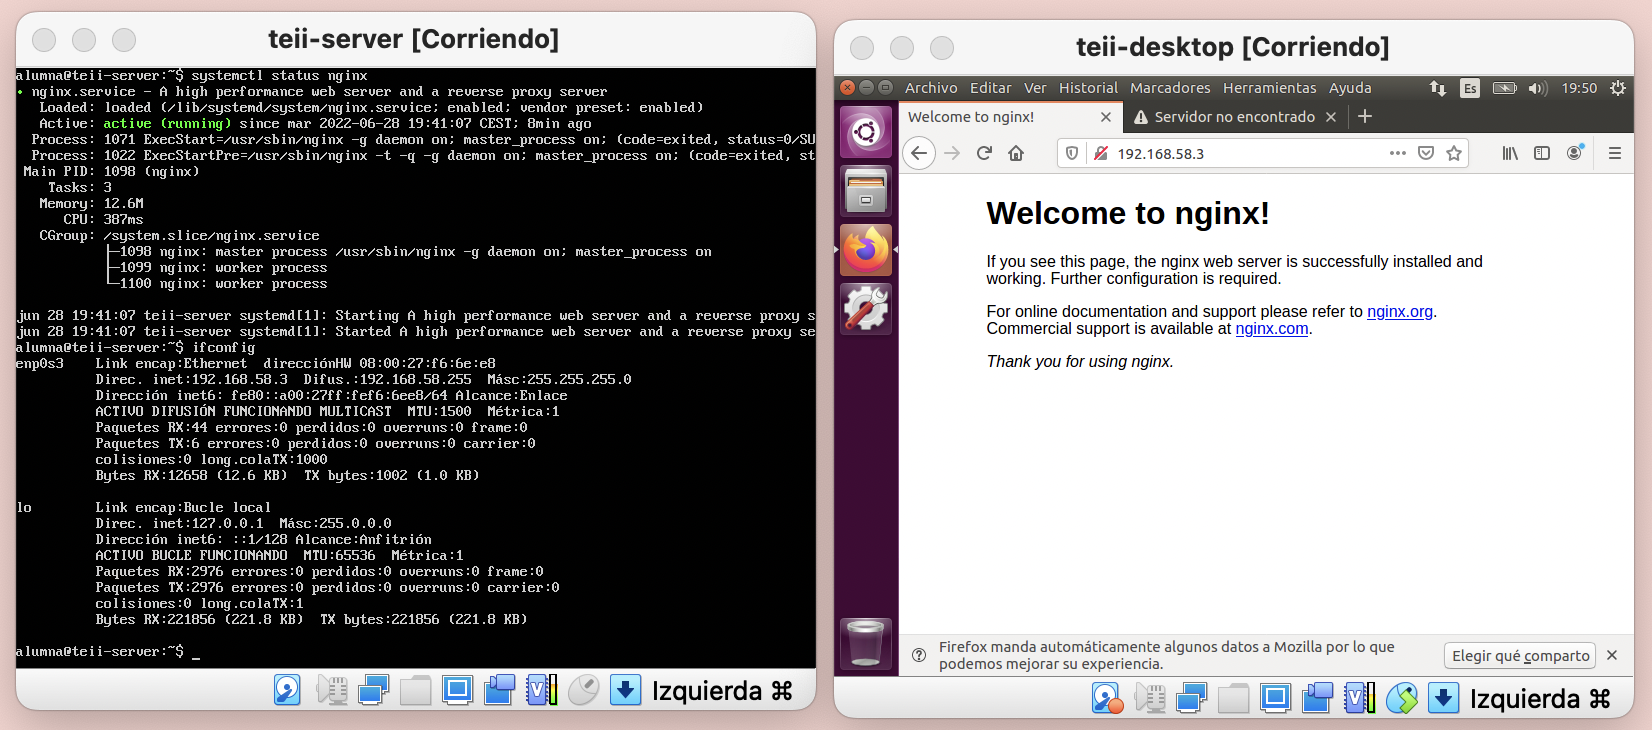
\includegraphics[width=\textwidth]{comprobacion-desktop}
    \centering
    \caption{Comprobación acceso al servidor web \textit{teii-server} desde la VM \textit{teii-desktop}.}
    \label{fig:comprobacion-desktop}
\end{figure}

%%%%%%%%%%%%%%%%%%%%%%%%%%%%%%%%%%%%%%%%%%%%%%%%%%%%%%%%%%%%%%%%%%%%%%%%%%%%%%%%%%%%%%%%%%%%%%%%%%%%%%%%%%%%%%%%%%%%%%%%%%%%%%%%%%%%%%%%%%%%%%
\subsubsection{Transformar el disco de la máquina de formato .vdi a formato qcow2.}

\begin{listing}[style=consola]
    $ 
\end{listing}


%%%%%%%%%%%%%%%%%%%%%%%%%%%%%%%%%%%%%%%%%%%%%%%%%%%%%%%%%%%%%%%%%%%%%%%%%%%%%%%%%%%%%%%%%%%%%%%%%%%%%%%%%%%%%%%%%%%%%%%%%%%%%%%%%%%%%%%%%%%%%%
\subsubsection{Redimensionar la maquina original servidor de VirtualBox con la utilidad Vboxmanage: 2GB de RAM y 10GB disco duro.} 

\begin{listing}[style=consola]
    $ 
\end{listing}


%%%%%%%%%%%%%%%%%%%%%%%%%%%%%%%%%%%%%%%%%%%%%%%%%%%%%%%%%%%%%%%%%%%%%%%%%%%%%%%%%%%%%%%%%%%%%%%%%%%%%%%%%%%%%%%%%%%%%%%%%%%%%%%%%%%%%%%%%%%%%%
\subsubsection{Destruir las máquinas virtuales (utilizando comandos).}

\begin{listing}[style=consola]
    $ 
\end{listing}



\begin{comment}
\subsection{Enunciado libvirt/kvm}
//TODO: Cambiar algunas cosas que son relativas a VirtualBox y no a esto
\begin{ejer}
    \par El objetivo de esta práctica es gestionar máquinas virtuales con el hipervisor libvirt/kvm. 
	Para ello se deberán realizar las siguientes tareas:
	\begin{itemize}
		\item Crear una VM mediante libvirt/kvm, Vboxmanage: 
		\begin{itemize}
			\item 1GB de ram, 2 cpus, 8 GB de disco duro SATA.
		\end{itemize}
		\item Instalar ubuntu-server en la máquina. Instalarle el servicio nginx a la máquina. 
		\item Instalar Ubuntu-desktop en otra máquina. Instalar un navegador web. 
		\item Comprobar que podemos acceder al servidor web desde un navegador en el host 
		\item Comprobar que podemos acceder al servidor web desde un navegador en la máquina guest desktop.
		\item Transformar el disco de la máquina de formato .vdi a formato qcow2. 
		\item Redimensionar la maquina original servidor de libvirt/kvm con la utilidad \textbf{Vboxmanage:} 2GB de RAM y 10GB disco duro. 
		\item Destruir las máquinas virtuales (utilizando comandos).
	\end{itemize}
\end{ejer}



\subsection{Segundo contenedor: mostrar la hora actual por pantalla.}


\subsubsection{Creación imagen hora}
\par Existen imágenes oficiales, pero en este caso creo una sencilla a partir de una de ellas.
La creación de esta imagen es exactamente igual que la anterior cambiando el nombre del script.
\par \textbf{Dockerfile2}
\begin{listing}
    # 2 capas de esta nueva imagen
    FROM ubuntu
    
    # Puede ir en cualquier nivel de la imagen, normalmente al inicio
    LABEL version=1.0
    LABEL description="Muestra la hora actual por pantalla cada segundo." 
    LABEL vendor=elenatablas
    
    COPY hora.sh /hora.sh
    ENTRYPOINT ["/hora.sh"] 
\end{listing}

\par \textbf{hora.sh}
\par Este script muestra la hora cada segundo durante su ejecución.
\begin{listing}
    #!/bin/bash

    while true; do echo "$(date +%T)"; sleep 1; done 
\end{listing}

\end{comment}

\subsection{Enunciado Vagrant}
\begin{ejer}
    \par El objetivo de esta práctica es gestionar máquinas virtuales con el hipervisor Vagrant. 
	Para ello se deberán realizar las siguientes tareas:
	\begin{itemize}
		\item Crear una Box de Vagrant. 
		\item Configurar el servidor Apache con Vagrant en la VM creada (Usar el provider Shell de Vagrant para configurar e instalar el Apache automáticamente al crear la VM).
		\item Redimensionar con Vagrant la máquina a 2GB de RAM y 2 CPUs.
		\item Comprobar que podemos acceder desde la máquina virtual creada con Vagrant al servidores web de la otra máquina virtual creada con VboxManage y viceversa.
	\end{itemize}
\end{ejer}



\subsection{Tercer contenedor: generar un número aleatorio y mostrarlo por pantalla.}

\subsubsection{Creación imagen numero}
\par Existen imágenes oficiales, pero en este caso creo una sencilla a partir de una de ellas.
La creación de esta imagen es exactamente igual que las anteriores cambiando el nombre del script.
\par \textbf{Dockerfile3}
\begin{listing}
    # 2 capas de esta nueva imagen
    FROM ubuntu
    
    # Puede ir en cualquier nivel de la imagen, normalmente al inicio
    LABEL version=1.0
    LABEL description="Muestra un numero aleatorio por pantalla cada segundo." 
    LABEL vendor=elenatablas
    
    COPY numero.sh /numero.sh
    ENTRYPOINT ["/numero.sh"] 
\end{listing}

\par \textbf{numero.sh}
\par Este script genera y muestra un número aleatorio cada segundo durante su ejecución.
\begin{listing}
    #!/bin/bash

    while true; do echo $(($RANDOM)); sleep 1; done  
\end{listing}